\chapter{Cascade of Transducers}
\label{chap-cassys}

This chapter presents the tool \textit{Cassys} that provides users the possibility to create Unitex cascade of transducers and new opportunities to work on natural language whith Finite State Graphs. A \textit{cascade of transducers} \index{cascade of transducer} applies several FSGraphs (also called automata or transducers), one after the other, onto a text: each graph modifies the text, and changes can be useful for further processings with the next graphs. Such a system is typically used for syntactic analysis, chunking, information extraction, recognizing named entities etc. To do that, CasSys uses a succession of "locate patterns" to which was added special options and behaviors.

\bigskip
\noindent The first prototype of the \textit{CasSys} \index{CasSys} system was created in 2002 at the LI 
(Computer science Laboratory of Universit� Fran�ois Rabelais Tours, France) \cite{these-nathalie}. This prototype was totally  dedicated to named entity recognition. Later, CasSys was generalized to allow any sort of work needing a cascade: throughout the years,  it was improved but never really integrated in Unitex, until a recent project which resulted in the complete integration of CasSys in Unitex\footnote{"Feder-R�gion Centre Entit�s  nomm�es et nommables" managed by Denis Maurel, LI, Tours, France, integration carried out by Nathalie Friburger and David Nott}.


Unitex grammars are known as Context free grammars and contain the notion of transduction derived from the field 
of finite state automata. A grammar with transduction (a transducer) is enabled to produce some ouput. 
Cassys is dedicated to the application of transducers in the form of a cascade.

\bigskip
A cascade can be used for syntactic analysis, chunking, information extraction, etc. 
\noindent Transducers are interesting because they allow the association of a recognized sequence to informations found in the outputs of the graphs. 
These outputs can:
\begin{itemize}
	\item	Be merged with the recognized sequence and appear in the resulting concordance or modified text. 
	\item	Replace the recognized sequence to modify the text. 
\end{itemize}
\noindent These two operations transform the text or add information inside the text. 


\bigskip
\noindent  
In this chapter, we will explain how to create/modify cascades of transducers and how to apply them. Then, we deals with options and behaviors offered by CasSys.

%%%%%%%%%%%%%%%%%%%%%%%%%%%%%%%%%%%%%%%%%%%%%%%%%%%%%%%%%%%%%
\section{Applying a cascade of transducers with CasSys}
\label{section:applyCascade}
Applying a cascade of transducers consists in the modelling of linguistic phenomena in several transducers listed in a specific order to apply on a text: CasSys and its interface into Unitex permits to do this. This section explains how to use the interface to create, manage (order, add, delete) graphs and apply the cascade.   

%%%%%%%%%%%%
\subsection{Creating the list of transducers}
\label{subsec:listTrans}

\bigskip
\noindent 
In order to manage the list of transducers, the menu FSGraph proposes two submenus: "\textit{New cascade}" and "\textit{Edit cascade...}" (Figure \ref{fig13-08}). You can choose "\textit{new cascade}" to create a new list of transducers. If you want to modify an existing cascade, you can choose "\textit{Edit cascade}" that open a file explorer to choose the cascade to open. 

\begin{figure}[!htb]
 \centering
 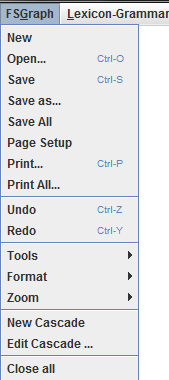
\includegraphics[width=4cm]{resources/img/fig13-08.png}
 \caption{"FSGraph" menu of Unitex and submenus "\textit{New cascade}" and "\textit{Edit cascade...}"}
 \label{fig13-08}
\end{figure}

In the language folder, there is a folder named CasSys where the cascade configuration files are stored. Those files are text files with the extension \textit{.csc} (ex: mycascade.csc).

%%%%%%%%%%%%
\subsection{Editing the list of transducers}
\label{subsec:editlistTrans}

The Cassys configuration window (Figure \ref{fig13-03}) is divided into three parts :

\begin{figure}[!htb]
  \centering
  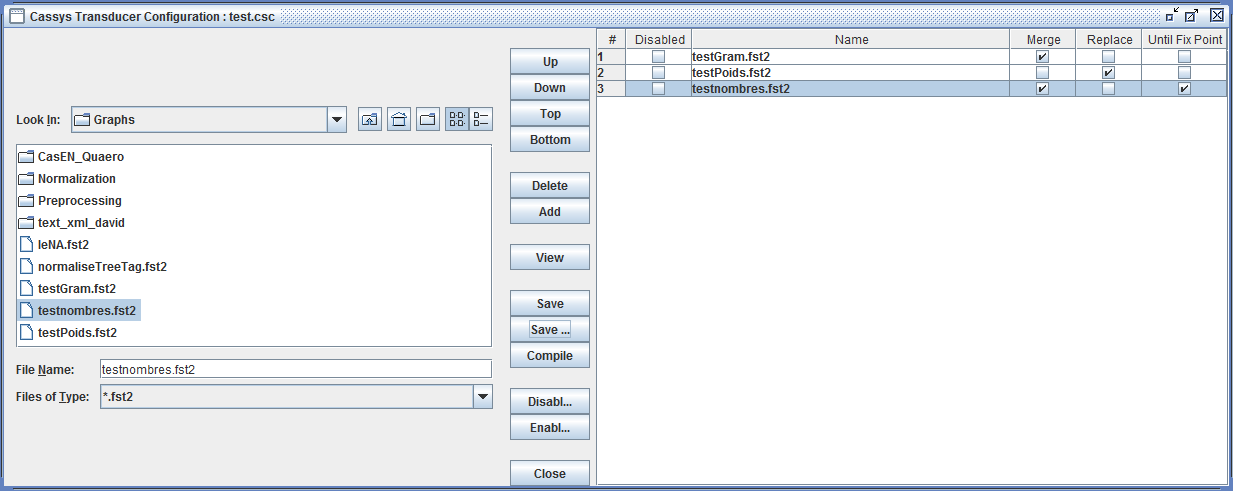
\includegraphics[width=16cm]{resources/img/fig13-03.png}
  \caption{Cassys configuration window with a list of transducers on the right hand side}
  \label{fig13-03}
\end{figure}

\begin{enumerate}
	\item a \textit{file explorer} at the left of the frame permits to select the transducers to place in the cascade. 
	The file explorer only displays fst2 files (all the graphs you want to place in the list of transducers must be compiled in fst2 format). 
	
	To edit the cascade, select the graphs in the file explorer at the left and drag and drop them into the right frame of the window.
	\item A \textit{table} at the right displays the cascade: the ordered list of transducers and the selected options for each graph.
		This table is obviously empty for a new cascade. 
	 
	The different columns of this table (Figure \ref{fig13-09}) show the numbering of each graph and permit to choose its behavior:
	\begin{itemize}
		  \item \textbf{\#}: Rank of the graph/transducer in the cascade. The resulting file of a graph is numbered with this rank.
		  \item \textbf{Disabled}: checkbox to disable the current graph. \textit{Disabled} meaning "\textit{not applied in the cascade}". The disabled graphs appear not numbered, in light grey and striked out.
			\item \textbf{Name}: The name of the graph (with extension \emph{fst2}). If you let the mouse over the name of the graph, a tooltip appears with the whole path ot the graph. Graphs which source file are not found appear in italic red font style.
		  \item \textbf{merge}: Whether the transducer should be applied in merge mode at the sense of unitex locate pattern.
			\item \textbf{replace}: Whether the transducer should be applied in replace mode at the sense of unitex locate pattern.
		  \item \textbf{iter}: Whether the transducer should be applied once or re-applied several times until no change occur in the text (See \ref{sub:AppWhiCon}).
	\end{itemize}

	\item \textit{Several buttons} in the middle for different needs: 
		\begin{itemize}
			\item \textit{"Up/Down/Top/Bottom"} buttons are used to modify the order of the transducers on the list (it moves the selected transducer in the list); 
			\textit{"Up"} and \textit{"Down"} to move the selected transducer one line up or down, and "Top" and "Bottom" to move the selection to the top or to the end of the list.
			\item  \textit{"Delete"} permits to remove a selected transducer from the list of transducers. 
			\item		\textit{"Add"} adds a transducer (previously selected in the explorer) onto the list. It replaces the drag and drop actions described above. 
			\item \textit{"View"} opens the selected graph either in the file explorer or in the list of transducers of the window. It is very useful to get a quick access to any transducer either to take a quick look at its content or to modify it.
			\item \textit{"Save"} and \textit{"Save as"} permit to save the list of transducers. By default, the lists of transducers are stored in the CasSys folder of the current language (e.g. English/Cassys).
			\item \textit{"Compile"} recompile all the graphs of the cascade. Very useful to avoid to recompile a graph after changes.
			\item \textit{"Disable all"} to disable all the graphs of the cascade. 
			\item \textit{"Enable all"} to enable all the graphs of the cascade. 
			\item \textit{"Close"} to close the current window.
		\end{itemize}
\end{enumerate}

\begin{figure}[!htb]
  \centering
  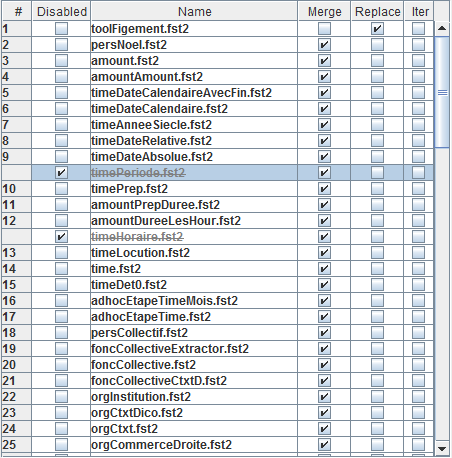
\includegraphics[width=7cm]{resources/img/fig13-09.png}
  \caption{The table/list of transducers}
  \label{fig13-09}
\end{figure}

	
%%%%%%%%%%%%%%%%%%%
\subsection{Applying a cascade}
\label{subsec:launchCascade}

To apply a cascade on a text, you can select the menu "\textit{Text / Apply CasSys cascade...}" (Figure \ref{fig13-01}) which will open the CasSys window.
This submenu "\textit{Apply CasSys cascade...}" is active only if a text has previously been opened.

\begin{figure}[!htb]
 \centering
 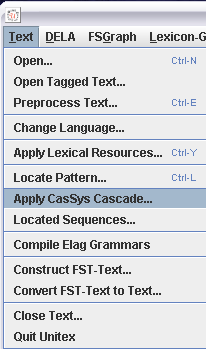
\includegraphics[width=5cm]{resources/img/fig13-01.png}
 \caption{"\textit{Text}" menu of Unitex and submenu "\textit{Apply CasSys Cascade...}"}
 \label{fig13-01}
\end{figure}


The CasSys window (Figure \ref{fig13-02}) displays the content of the CasSys folder of the current language. It permits to let you choose 
the cascade file you want to apply on the text. When this list is chosen, you can click on the "Launch" button to apply the cascade.

\begin{figure}[!htb]
  \centering
  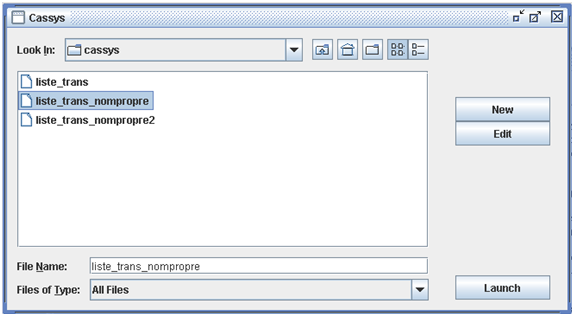
\includegraphics[width=10cm]{resources/img/fig13-02.png}
  \caption{CasSys Window to launch a cascade of transducers}
  \label{fig13-02}
\end{figure}


Note that any morphological dictionnaries added in your preferences is applied to your
graphs. This preferences may be edited from the main unitex frame (\textit{info / Preferences / morphological dictionnaries}).

\subsection{Sharing a cascade transducer list file}
\label{subsec:shareCascade}

In order to ease collaborating work within CasSys, a  simple export/import
system for the cascades is provided. This possibility is offered in the "\textit{Text / Apply CasSys cascade...}" menu.

To share a cascade list file, the following steps has to be fullfilled :
\begin{enumerate}
  \item \textbf{Export :} Select a cascade file and click the export button. (A
  ready to share file is created in the \texttt{/Cassys/Share} repository)
  \item Send the file to share to your colleague
  \item \textbf{Import :} Select the imported file and click the import button.
  (A ready to use file is created in the \texttt{/Cassys} repository)
\end{enumerate}


%%%%%%%%%%%%%%%%%%%%%%%%%%%%%%%%%%%%%%%%%%%%%%%%%%%%%%%
\section{Details on the behavior of Cassys}

In this section , we present details concerning the functioning of Cassys.

%%%%%%%%%%%%%
\subsection{Type of graphs used}

Cassys uses the compiled version of the graphs (the fst2 files).
Cassys can handle the local grammars (section 6.1) (syntactic graphs) presented in Chapter \ref{chap-advanced-grammars}. These grammars can use subgraphs, morphological filters and mode, and allow to refer to information in dictionaries. 
The grammars used in the cascade must follow the constraints of the grammars used in Unitex.

\subsection{Apply while concordance behaviour}
\label{sub:AppWhiCon}

Cassys may apply a transducer on a text while concordances are found. This behavior is selected if the checkbox \textbf{iter} is checked or not for each graph of a cascade.
\bigskip
For instance, consider the very simple graph \ref{fig:AB->A} which recognizes \emph{AB} and
replaces it with \emph{A}. 

\begin{figure}[!htb]
  \centering
  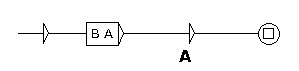
\includegraphics[width=7cm]{resources/img/AB_to_A.png}
  \caption{Transducer which modifies BA in A}
  \label{fig:AB->A}
\end{figure}

Consider the text \emph{B B B A A A}. Applying the graph \ref{fig:AB->A} onto this text with \emph{iter} will have the following result :\\

\begin{tabular}{|l|cccccc|r|}
\hline
initial text  &B&B&B&A&A&A&\\
\hline
iteration 1 & &B&B&A&A&A& 1 match\\
iteration 2 & & &B&A&A&A& 1 match\\
iteration 3 & & & &A&A&A& 1 match\\
iteration 4 & & & &A&A&A& 0 match\\
\hline
\end{tabular} \\

During the three first iterations, a match is found, so the graph
re-applied on the resulting text. At the fourth iteration, no match is
found, so the graph is not re-applied.

\large{\textbf{Warning:}} Be aware of the risk of livelock when applying this
option. For example, a transducer which recognizes \emph{A} and replaces it with
\emph{A} would be caught in a livelock if applied on the example text.

%%%%%%%%%%%%%%%%%%%%
\subsection{The Unitex rules used for the cascade}

In the cascade, each successive graph is applied following the unitex rules:
\begin{itemize}
	\item \textit{Insertion to the left of the matched patterns}: in the merge mode, the ouput is inserted to the left of the recognized sequence.
	\item	\textit{Priority of the leftmost match}: during the application of a local grammar, overlapping occurrences are all indexed. 
	During the construction of a concordance, all these overlapping occurrences are presented but CasSys modifies the text with each 
	graph of the cascade : so it is necessary to choose among these occurrences the one that will be taken into account. To do that, the priority is given to the leftmost sequence.
	\item \textit{Priority of the longest match}: in CasSys, during the application of a graph, it is the longest sequence 
	that will be kept.
	\item	\textit{Search limitation to a certain number of occurrences}: in Cassys, this search is not limited. Such a limitation has no sense in the use of CasSys, we allways index all utterances in the text.
\end{itemize}

%%%%%%%%%%%%%%%%%%%%
\subsection{A special way to mark up patterns with CasSys}

The output of the transducers can be used to insert special information into texts, particularly to mark up the recognized patterns: it is 
possible to use all the marks you want such as ( ), [], "", etc. or xml tags such as <xxx> </xxx>.\\
Cassys also offers\textit{ a special way to mark up patterns}, that offers some advantages and that we present here.  

\bigskip
\noindent Unitex splits texts into different sorts of tokens like the sentence delimiter {S}; the stop marker {STOP}, contiguous 
sequences of letters, lexical tags {aujourd'hui,.ADV}, etc.//
The lexical tag is used by CasSys in a special way. The lexical tag (between curly brackets) is normally used to avoid ambiguities (see section \ref{tokenization} and section\ref{section-displaying-sentence-automata}). 
For example, if the token \emph{\{curly brackets,.N\}} is in a text, neither "curly" nor "brackets" will be recognized but the whole sequence 
"curly brackets" or the tag <N>.// 
A lexical tag can contain complex lexical information. For example, the codes \emph{N+Pers+Hum:fs} tags a token which is a noun, a person, a human and feminine singular. In a graph, you can look for a lexical token using the lexical codes it contains: for example, you can write lexical masks such as \emph{<N>} to search a noun, \emph{<Pers+Hum>} for a human person or simply \emph{<Pers>} (lexical masks are explained in section \ref{section-special-symbols}).
 
\bigskip
\noindent In Cassys, we use the lexical tag in a special way. A cascade of transducers is interesting to locate the island of certainty first. It is necessary for such a system to avoid that previously recognized patterns be ambiguous with patterns recognized by the following graphs. To do that, you can tag the patterns of your graphs surrounding them by \emph{\{} and \emph{,.tag1+tag2+tagn\}} in the outputs of the graph (where \emph{tag1, tag2, etc.} are your own tags).

\bigskip
\noindent To explain this behavior, here is a very simple example. The text on which we work is :

\emph{bac a b c cc a b b ba ab a b bca a b c abaabc}.

\bigskip
\noindent The graph grfAB (\ref{fig13-05}) recognizes the sequence \emph{a b} in the text and tags this sequence with the lexical tag \textit{\{a b,.AB\}}. The results are merged with the text adding the outputs \emph{\{ }and \emph{,.AB\}} around \textit{"a b"} sequences. 

\begin{figure}[!htb]
  \centering
  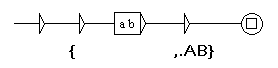
\includegraphics[width=6cm]{resources/img/fig13-05.png}
  \caption{The graph grfAB}
  \label{fig:fig13-05}
\end{figure}

\bigskip
\noindent The resulting text is : \emph{bac \{a b,.AB\} c cc \{a b,.AB\} b ba ab \{a b,.AB\} bca \{a b,.AB\} c abaabc}.

\bigskip
\noindent Now the pattern \emph{a b} is tagged \emph{AB}. A part (a or b alone) of this pattern cannot be recognized because of the tagging of \emph{a b}. 

\bigskip
\noindent After that graph, the cascade applies another graph named tagAB (\ref{fig13-06}). iI has two paths: 
\begin{itemize}
	\item the first one to recognize the lexical mask \textit{<AB>} followed by \textit{c} and tags this sequence as \textit{ABC}.
  \item the second one to recognize and tag \textit{bca} preceeded by \textit{<AB>}. Only \textit{bca} is tagged as \textit{BCA}.
\end{itemize}

\begin{figure}[!htb]
  \centering
  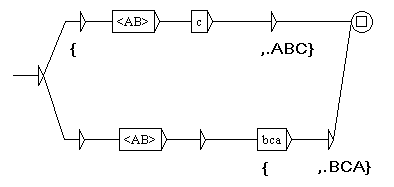
\includegraphics[width=9cm]{resources/img/fig13-06.png}
  \caption{The graph tagAB}
  \label{fig13-06}
\end{figure}

\bigskip
\noindent The resulting text is : \emph{bac \{\{a b,.AB\} c,.ABC\} cc \{a b,.AB\} b ba ab \{a b,.AB\} \{bca,.BCA\} \{\{a b,.AB\} c,.ABC\} abaabc}.

% \#M
% 2.0.0 6.0.0 \{\\\{a b\\,\\.AB\\\} c,.ABC\}
% 10.0.0 12.0.0 \{a b,.AB\}
% 20.0.0 24.2.0 \{a b,.AB\} \{bca,.BCA\}
% 26.0.0 30.0.0 \{\\\{a b\\,\\.AB\\\} c,.ABC\}

\bigskip
\noindent The concordance displayed by Unitex should be like in (\ref{fig13-07}). //

Note that for programming reasons (ambiguities between characters in the curly brackets of the lexical tags), we have no option but to place backslashes $\backslash$ before all ambiguous characters for Unitex ; that is why these symbols are protected with $\backslash$ in the concordance to avoid problems in Unitex. 

\begin{figure}[!htb]
  \centering
  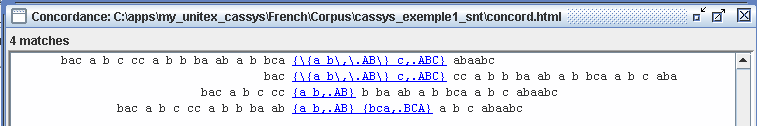
\includegraphics[width=15cm]{resources/img/fig13-07.png}
  \caption{The concordance resulting from this cascade}
  \label{fig13-07}
\end{figure}


%%%%%%%%%%%%%%%%%%%%%%%%%%%%%%%%%%%%%%%%%%%%%%%%%%%%%%%%%%%%%%
\section{The results of a cascade}

%%%%%%%%%%%%%%%%
\subsection{Displaying the concordance of a cascade}
\label{subsec:resultsCascade}

The results of a cascade are stored in an index file (concord.ind), just as for the \textit{"Locate pattern"} operation. This index file contains all the sequences recognized using the restrictions imposed by the rules of unitex.

\bigskip
\noindent In order to display a concordance, you have to access the frame "\textit{Text / Located sequences...}" and click on the "\textit{Build concordance}" button (as described in Chapter \ref{chap-advanced-grammars}).
The figure \ref{fig13-04} presents a sample of concordance resulting of a cascade recognizing named entities. 
\begin{figure}[!htb]
  \centering
  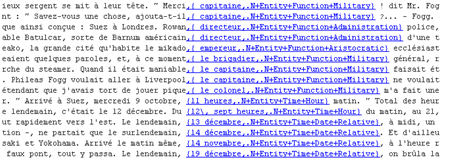
\includegraphics[width=14cm]{resources/img/fig13-04.png}
  \caption{Concordance of Cassys under Unitex}
  \label{fig13-04}
\end{figure}

%%%%%%%%%%%%
\subsection{The different resulting files of a cascade}

Cassys keeps all the text created by each graph of the cascade. This can be useful to test, debug or check the different results of the cascade. It is possible to correct the errors on the order of the graphs or to find the errors in the writing of the graphs. A good idea is to write the name of the graph recognizing a pattern in the output of this graph: thanks to that, you can see in the final results the name of the graph by which a pattern is recognized. 
\bigskip

If you apply a cascade on the text named \texttt{example.txt}, two folders are created: \texttt{example\_snt} and \texttt{example\_csc}.
The files produced in \texttt{example\_csc} are the results obtained by each graphs. These files are named according to the number of the graph which produced them. For example, if the third graph of a cascade finds at least a pattern, the results of this graph will be stored in the folder \texttt{example\_3\_0\_snt} and the file named \texttt{example\_3\_\0.snt} will contain the modified text.

%%%%%%%%%%%
\subsection{An xml-like output text for lexical tags}

As an output, the lexical tag format is transformed into an xml-like format.
This change is done in order to provide an easier-to-manipulate text to the end
user. 
From this format, it is possible to use one of the numerous tools to process xml or it is easier to apply further transducers to get the output anyone
wants.\\
This xml-ized ouput text is copied in the file \texttt{example\_csc.txt} while the raw text is in the file \texttt{example\_raw.txt}.

More precisely, The lexical tag has the following format :\\
\begin{tabular}{c}
\texttt{
\{forme.lemme,code1+code2:flex1:flex2\}}
\end{tabular}\\

The xml-like outputs of cassys has the following format :\\
\begin{tabular}{ll}
\texttt{<csc>}&\\
	&\texttt{<form>forme</form>}\\
	&\texttt{<lem>lemme</lem>}\\
	&\texttt{<code>code1</code>}\\
	&\texttt{<code>code2</code>}\\
	&\texttt{<inflect>flex1</inflect>}\\
	&\texttt{<inflect>flex2</inflect>}\\
\texttt{</csc>}&\\
\end{tabular}

The DTD corresponding to our xml format is:

\begin{tabular}{l}
\texttt{<?xml version="1.0" encoding="ISO-8859-1"?>}\\
\texttt{<!ELEMENT text (#PCDATA|csc)* >}\\
\texttt{<!ELEMENT csc (form,lem?,code*,inflect*) >}\\
\texttt{<!ELEMENT form (#PCDATA|csc)*>}\\
\texttt{<!ELEMENT lem (#PCDATA)>}\\
\texttt{<!ELEMENT code (#PCDATA)>}\\
\texttt{<!ELEMENT inflect (#PCDATA)>}\\
\end{tabular}


